\documentclass[12pt,a4paper]{article}
\usepackage[a4paper,top=12mm,bottom=14mm,left=15mm,right=15mm]{geometry}
\usepackage[T1]{fontenc}
\usepackage{amsmath}
\usepackage{amssymb}
\usepackage{enumitem}
\usepackage{multicol}
\usepackage{xcolor}
\usepackage{tikz}
\usepackage[most]{tcolorbox}
\usetikzlibrary{decorations.pathreplacing,arrows.meta}

% ================================================================
% Recurring decimals to fractions.
%
% An extension sheet for the top end of a middle ability Year 9
% class, designed to be worked through alone: every method is
% introduced by a worked example, practised once with the steps
% written out, and then practised without them. Answers are on the
% last page so that pupils can check each part before going on.
%
% The sheet is written on, so it is set with open leading and wide
% list separation, and every question is followed by a working area
% sized to fill the rest of its page. The \newpage commands in the
% body are placed so that no question is ever split across the fold;
% because of them a part may run to more than one page.
% ================================================================

\pagestyle{empty}
\linespread{1.2}\selectfont
\setlength{\parskip}{5pt}
\renewcommand{\arraystretch}{1.35}
\setlist[enumerate,1]{label=\textbf{Q\arabic*.}, leftmargin=*, itemsep=12pt, topsep=8pt, parsep=4pt}
\setlist[enumerate,2]{label=(\alph*), leftmargin=*, itemsep=8pt, topsep=5pt, parsep=3pt}
\setlength{\multicolsep}{8pt}
\setlength{\parindent}{0pt}

\newcommand{\ansline}[1][2.2cm]{\underline{\hspace{#1}}}

% A worked example: the method shown in full before it is practised.
\newtcolorbox{wex}[1]{colback=blue!4,colframe=blue!45!black,boxrule=0.6pt,
  left=6pt,right=6pt,top=4pt,bottom=5pt,
  title={\bfseries\small Worked example: #1},fonttitle=\small,
  toptitle=1pt,bottomtitle=1pt}

% The idea a section is built on, stated once and boxed.
\newtcolorbox{keyidea}{colback=orange!7,colframe=orange!60!black,boxrule=0.6pt,
  left=6pt,right=6pt,top=4pt,bottom=4pt}

% The section headings, kept tight so the parts do not eat the page.
\newcommand{\heading}[1]{%
  \vspace{2pt}
  {\color{blue!45!black}\rule{\linewidth}{1pt}}\\[1pt]
  {\large\bfseries #1}\\[-6pt]
  {\color{blue!45!black}\rule{\linewidth}{0.4pt}}
  \vspace{2pt}}
\newcommand{\parttitle}[2]{\heading{Part #1: #2}}

% ----------------------------------------------------------------
% One line of a subtraction diagram. Every row puts its decimal
% point at the same x, so that recurring tails which really are
% identical end up in the same columns on the page.
% \drow{<y>}{<label>}{<digits before the point>}{<digits after>}
\newcommand{\drow}[4]{%
  \node[anchor=east,font=\small] at (-1.25,#1) {#2};
  \node[anchor=east,font=\small] at (-0.12,#1) {#3};
  \node[font=\small] at (0,#1) {.};
  \foreach \d [count=\i from 0] in {#4}
    {\node[font=\small] at ({0.34+\i*0.34},#1) {\d};}%
}
% The band of columns from digit #1 to digit #2, used to shade a tail.
\newcommand{\tailbox}[4]{%
  ({0.34+#1*0.34-0.17},#3) rectangle ({0.34+#2*0.34+0.17},#4)}
% The same row as \drow, but with a writing line in each digit column so that
% a pupil fills the row in. #4 is how many columns to draw before the dots.
% \drowgap{<y>}{<label>}{<before the point>}{<number of columns>}
\newcommand{\drowgap}[4]{%
  \node[anchor=east,font=\small] at (-1.25,#1) {#2};
  \node[anchor=east,font=\small] at (-0.12,#1) {#3};
  \node[font=\small] at (0,#1) {.};
  \foreach \i in {1,...,#4}
    {\draw[gray!60] ({0.34+(\i-1)*0.34-0.13},{#1-0.16}) --
                    ({0.34+(\i-1)*0.34+0.13},{#1-0.16});}
  \node[font=\small] at ({0.34+#4*0.34},#1) {$\ldots$};%
}
% Solving by dividing both sides: the equation before above the equation
% after, with a curved arrow down each side carrying the division. Both
% arrows bend outwards, so neither crosses the equation.
% \divideboth{<lhs>}{<rhs>}{<new lhs>}{<new rhs>}{<divisor>}
\newcommand{\divideboth}[5]{%
  \begin{tikzpicture}
    \node (tl) at (0,0)     {$#1$};
    \node       at (0.7,0)  {$=$};
    \node (tr) at (1.5,0)   {$#2$};
    \node (bl) at (0,-1.5)  {$#3$};
    \node       at (0.7,-1.5) {$=$};
    \node (br) at (1.5,-1.5) {$#4$};
    \draw[-{Stealth[length=2mm]},blue!45!black] (tl) to[bend right=65]
      node[left=1pt,font=\scriptsize]{$\div\,#5$} (bl);
    \draw[-{Stealth[length=2mm]},blue!45!black] (tr) to[bend left=65]
      node[right=1pt,font=\scriptsize]{$\div\,#5$} (br);
  \end{tikzpicture}%
}

\begin{document}

\begin{center}
  {\Large\bfseries Recurring Decimals into Fractions}\\[8pt]
\end{center}
\vspace{1pt}

\begin{keyidea}
\small
Every recurring decimal --- however long and however complicated --- can be written as a fraction. Follow the examples in this sheet to learn how to convert recurring decimals to fractions.
\end{keyidea}

\parttitle{1}{Reading and writing recurring decimals}

When you divide one whole number by another, the digits after the point either
stop, or fall into a block that repeats forever. Repeating blocks are marked with a dot over the \textbf{first} digit and a dot over the \textbf{last}
digit.

\begin{center}
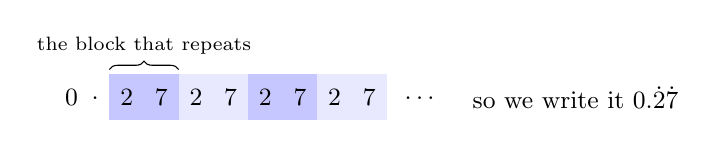
\begin{tikzpicture}[font=\small]
  \def\dgw{0.44}
  \foreach \s/\c in {0/blue!22, 2/blue!9, 4/blue!22, 6/blue!9}{
    \fill[\c] ({0.7+\s*\dgw-0.5*\dgw},-0.28) rectangle ({0.7+(\s+2)*\dgw-0.5*\dgw},0.3);}
  \node at (0,0) {$0$};
  \node at (0.3,0) {.};
  \foreach \d [count=\i from 0] in {2,7,2,7,2,7,2,7}
    {\node at ({0.7+\i*\dgw},0) {\d};}
  \node at ({0.7+8*\dgw+0.2},0) {$\ldots$};
  \draw[decorate,decoration={brace,amplitude=3pt}]
    ({0.7-0.5*\dgw},0.36) -- ({0.7+1.5*\dgw},0.36)
    node[midway,above=2pt,font=\scriptsize]{the block that repeats};
  \node[anchor=west,font=\small] at ({0.7+8*\dgw+0.75},0)
    {so we write it $0.\dot{2}\dot{7}$};
\end{tikzpicture}
\end{center}
\vspace{-4pt}

So $0.\dot{6}=0.6666666\ldots$, \; $0.\dot{2}\dot{7}=0.2727272\ldots$, \;
$0.\dot{4}0\dot{9}=0.4094094\ldots$ \; and $0.1\dot{6}=0.1666666\ldots$ ---
notice that in the last one only the $6$ carries a dot, so only the $6$
repeats. The $1$ only is found in the tenths column, and never comes back.

\vspace{2em}


\begin{enumerate}

\item Write out the first eight decimal places of each number.
\begin{multicols}{3}
\begin{enumerate}
  \item $0.\dot{5}=0.\ansline[2.3cm]$
  \item $0.\dot{1}\dot{8}=0.\ansline[2.3cm]$
  \item $0.3\dot{7}=0.\ansline[2.3cm]$
  \item $0.\dot{2}0\dot{6}=0.\ansline[2.3cm]$
  \item $0.4\dot{5}\dot{1}=0.\ansline[2.3cm]$
  \item $0.\dot{9}=0.\ansline[2.3cm]$
\end{enumerate}
\end{multicols}

\vspace{1em}

\item Write each of these using dot notation.
\begin{multicols}{3}
\begin{enumerate}
  \item $0.8888\ldots=\ansline[1.5cm]$
  \item $0.636363\ldots=\ansline[1.5cm]$
  \item $0.24444\ldots=\ansline[1.5cm]$
  \item $0.157157\ldots=\ansline[1.5cm]$
  \item $0.91666\ldots=\ansline[1.5cm]$
  \item $0.40505\ldots=\ansline[1.5cm]$
\end{enumerate}
\end{multicols}

\vspace{1em}

\item
\begin{enumerate}
  \item Which is bigger, $0.\dot{4}\dot{5}$ or $0.4\dot{5}$? Write both out to
        six decimal places to help you decide, and explain your answer.

        \vspace{7em}
  \item Write down a recurring decimal that lies between $0.\dot{3}$ and
        $0.\dot{4}$. \ansline[3cm]
\end{enumerate}

\end{enumerate}

% \parttitle{2}{The family of nines}

% Before any algebra, here is a pattern worth knowing. Use short division to
% check the first one or two, then follow the pattern.

% \begin{enumerate}[resume]

% \item Complete the following.
% \begin{multicols}{4}
% \begin{enumerate}
%   \item $\tfrac{1}{9}=0.\dot{1}$
%   \item $\tfrac{2}{9}=\ansline[1.4cm]$
%   \item $\tfrac{4}{9}=\ansline[1.4cm]$
%   \item $\tfrac{7}{9}=\ansline[1.4cm]$
% \end{enumerate}
% \end{multicols}

% \item Now with two and three nines on the bottom.
% \begin{multicols}{3}
% \begin{enumerate}
%   \item $\tfrac{1}{99}=0.\dot{0}\dot{1}$
%   \item $\tfrac{7}{99}=\ansline[1.8cm]$
%   \item $\tfrac{14}{99}=\ansline[1.8cm]$
%   \item $\tfrac{58}{99}=\ansline[1.8cm]$
%   \item $\tfrac{1}{999}=0.\dot{0}0\dot{1}$
%   \item $\tfrac{271}{999}=\ansline[1.8cm]$
% \end{enumerate}
% \end{multicols}

% \end{enumerate}

% \begin{keyidea}
% \small
% \textbf{The nines rule.} If a block of $n$ digits repeats \emph{straight after
% the decimal point}, the fraction is that block written over $n$ nines. So
% $0.\dot{8}=\tfrac{8}{9}$, \; $0.\dot{2}\dot{7}=\tfrac{27}{99}$ \; and \;
% $0.\dot{4}0\dot{9}=\tfrac{409}{999}$. Always simplify afterwards ---
% $\tfrac{27}{99}=\tfrac{3}{11}$.
% \end{keyidea}

% \begin{enumerate}[resume]

% \item Use the nines rule. Give each answer as a fraction in its simplest form.
% \begin{multicols}{3}
% \begin{enumerate}
%   \item $0.\dot{7}$ \ansline[1.6cm]
%   \item $0.\dot{2}\dot{4}$ \ansline[1.6cm]
%   \item $0.\dot{8}\dot{1}$ \ansline[1.6cm]
%   \item $0.\dot{6}$ \ansline[1.6cm]
%   \item $0.\dot{1}3\dot{5}$ \ansline[1.6cm]
%   \item $0.\dot{4}\dot{5}$ \ansline[1.6cm]
% \end{enumerate}
% \end{multicols}

% \end{enumerate}

% The nines rule is quick, but it only works when the repeating block starts
% immediately after the point --- it is no use at all on $0.1\dot{6}$ --- and it
% does not explain \emph{why} the nines appear. For both of those we need
% algebra, and that is the rest of the sheet.

\newpage

\parttitle{2}{Finding fractions from recurring decimals}

The trick is to find two numbers whose recurring tails are
\textbf{exactly the same}, and then subtract one from the other. The tails
cancel, and what is left has no decimals in it at all.

To do this we have to use an \textbf{algebraic variable}, which we will call $x$. $x$ stands for the recurring decimal we are trying to convert to a fraction.

\begin{wex}{turn $0.\dot{4}$ into a fraction}
\small
\textbf{Step 1 --- introduce $x$} We write $x=0.\dot{4}$, so $x=0.4444\ldots$

\smallskip
\textbf{Step 2 --- shift the place values.} Multiplying by $10$ moves every digit one place
to the left: \newline $10x=4.4444\ldots$ (remember $10x = 10 \times x$).

\smallskip
\textbf{Step 3 --- subtract.} The two tails are identical, so they cancel out when we subtract: $10x -x$.

\begin{center}
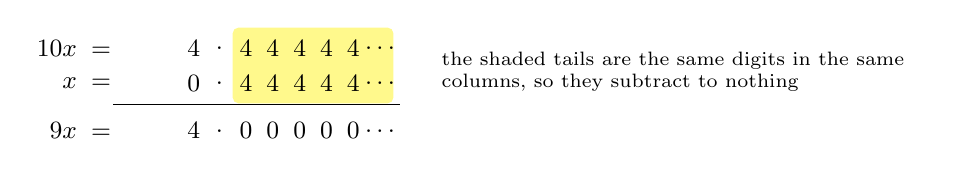
\begin{tikzpicture}[font=\small]
  \fill[yellow!45,rounded corners=2pt] \tailbox{0}{5}{-0.7}{0.26};
  \drow{0}{$10x\;=$}{$4$}{4,4,4,4,4,{$\ldots$}}
  \drow{-0.45}{$x\;=$}{$0$}{4,4,4,4,4,{$\ldots$}}
  \draw (-1.35,-0.72) -- (2.3,-0.72);
  \drow{-1.05}{$9x\;=$}{$4$}{0,0,0,0,0,{$\ldots$}}
  \node[anchor=west,font=\scriptsize,text width=6.2cm] at (2.7,-0.3)
    {the shaded tails are the same digits in the same columns, so they
     subtract to nothing};
\end{tikzpicture}
\end{center}
\vspace{-2pt}
So $10x-x=4$, which means $9x=4$.

\smallskip
\textbf{Step 4 --- solve.} We have $9$ lots of $x$, so we divide both sides
by $9$:

\vspace{-2pt}
\begin{center}
\divideboth{9x}{4}{x}{\dfrac{4}{9}}{9}
\end{center}
\end{wex}

\begin{enumerate}[resume]

\item Fill in the gaps to turn $0.\dot{7}$ into a fraction.

\textbf{Step 1 --- introduce $x$} We write $x=0.\dot{7}$, so
$x=\ansline[3.5cm]$

\smallskip
\textbf{Step 2 --- shift the place values.} Multiplying by $10$ moves every
digit one place to the left: \newline $10x=\ansline[3.5cm]$ (remember
$10x = 10 \times x$).

\smallskip
\textbf{Step 3 --- subtract.} The two tails are identical, so they cancel out
when we subtract: $10x-x$.

\begin{center}
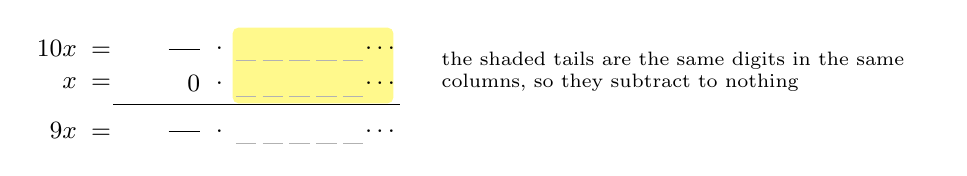
\begin{tikzpicture}[font=\small]
  \fill[yellow!45,rounded corners=2pt] \tailbox{0}{5}{-0.7}{0.26};
  \drowgap{0}{$10x\;=$}{\ansline[0.4cm]}{5}
  \drowgap{-0.45}{$x\;=$}{$0$}{5}
  \draw (-1.35,-0.72) -- (2.3,-0.72);
  \drowgap{-1.05}{$9x\;=$}{\ansline[0.4cm]}{5}
  \node[anchor=west,font=\scriptsize,text width=6.2cm] at (2.7,-0.3)
    {the shaded tails are the same digits in the same columns, so they
     subtract to nothing};
\end{tikzpicture}
\end{center}
\vspace{-2pt}
So $10x-x=\ansline[1.6cm]$, which means $9x=\ansline[1.6cm]$.

\smallskip
\textbf{Step 4 --- solve.} We have \ansline[0.9cm] lots of $x$, so we divide
both sides by \ansline[0.9cm]. Set your working out like the worked example.

\vspace{13em}

\newpage

\item Turn $0.\dot{8}$ into a fraction, using the same four steps.
\begin{itemize}[label={},leftmargin=1.8em,itemsep=12pt,topsep=6pt]
  \item \textbf{Step 1 --- introduce $x$} \hfill \ansline[7cm]
  \item \textbf{Step 2 --- shift the place values.} \hfill \ansline[7cm]
  \item \textbf{Step 3 --- subtract.} The two tails are identical, so they
        cancel out when we subtract: $10x-x$.
        \begin{center}
        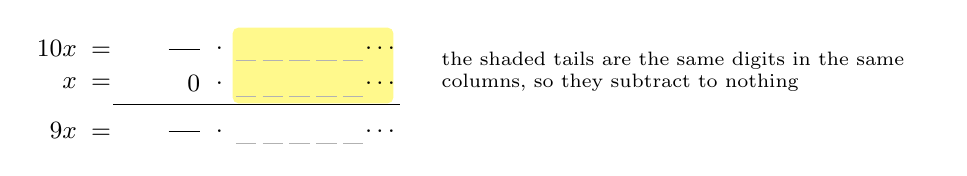
\begin{tikzpicture}[font=\small]
          \fill[yellow!45,rounded corners=2pt] \tailbox{0}{5}{-0.7}{0.26};
          \drowgap{0}{$10x\;=$}{\ansline[0.4cm]}{5}
          \drowgap{-0.45}{$x\;=$}{$0$}{5}
          \draw (-1.35,-0.72) -- (2.3,-0.72);
          \drowgap{-1.05}{$9x\;=$}{\ansline[0.4cm]}{5}
          \node[anchor=west,font=\scriptsize,text width=6.2cm] at (2.7,-0.3)
            {the shaded tails are the same digits in the same columns, so they
             subtract to nothing};
        \end{tikzpicture}
        \end{center}
        \vspace{-2pt}
        So $10x-x=\ansline[1.6cm]$, which means $9x=\ansline[1.6cm]$.
  \item \textbf{Step 4 --- solve.} Divide both sides by \ansline[0.9cm].

        \vspace{11em}
\end{itemize}

\item Turn each of these into a fraction in its simplest form. Write out all
four steps each time.
\begin{multicols}{4}
\begin{enumerate}
  \item $0.\dot{2}$
  \item $0.\dot{5}$
  \item $0.\dot{6}$
  \item $0.\dot{3}$
\end{enumerate}
\end{multicols}
\vspace{28em}

\end{enumerate}

\newpage

\parttitle{3}{Longer repeating blocks}

Try $0.\dot{3}\dot{6}$ the same way and the tails do not cancel. Multiplying by
$10$ shifts the place values by one, which puts the two digits of the block the
wrong way round. A block of \emph{two} digits has to be shifted by \emph{two}
place values, so we multiply by $100$ instead.

\vspace{4pt}
\begin{center}
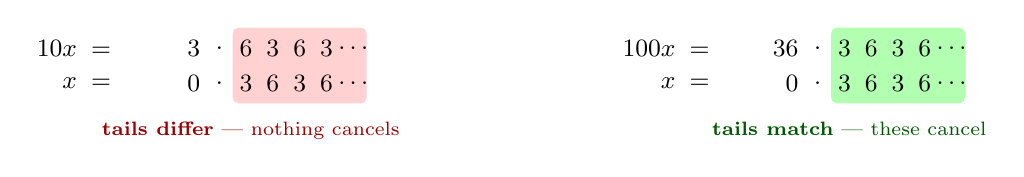
\begin{tikzpicture}[font=\small]
  \fill[red!18,rounded corners=2pt] \tailbox{0}{4}{-0.7}{0.26};
  \drow{0}{$10x\;=$}{$3$}{6,3,6,3,{$\ldots$}}
  \drow{-0.45}{$x\;=$}{$0$}{3,6,3,6,{$\ldots$}}
  \node[font=\scriptsize,anchor=north,red!60!black] at (0.4,-0.82)
    {\textbf{tails differ} --- nothing cancels};
  \begin{scope}[xshift=7.6cm]
    \fill[green!30,rounded corners=2pt] \tailbox{0}{4}{-0.7}{0.26};
    \drow{0}{$100x\;=$}{$36$}{3,6,3,6,{$\ldots$}}
    \drow{-0.45}{$x\;=$}{$0$}{3,6,3,6,{$\ldots$}}
    \node[font=\scriptsize,anchor=north,green!35!black] at (0.4,-0.82)
      {\textbf{tails match} --- these cancel};
  \end{scope}
\end{tikzpicture}
\end{center}
\vspace{4pt}

\begin{wex}{turn $0.\dot{3}\dot{6}$ into a fraction}
\small
\begin{tabular}{@{}ll@{\hspace{1.6em}}l@{}}
\textbf{Step 1 --- introduce $x$} & $x=0.\dot{3}\dot{6}$, so $x=0.363636\ldots$ & \\[8pt]
\textbf{Step 2 --- shift the place values.} & $100x=36.363636\ldots$
  & the block is $2$ digits long\\[8pt]
\textbf{Step 3 --- subtract.} & $100x-x=36$ & so $99x=36$\\[8pt]
\textbf{Step 4 --- solve.} & $x=\dfrac{36}{99}=\dfrac{4}{11}$ & \\
\end{tabular}
\end{wex}

\begin{enumerate}[resume]

\item Fill in the gaps to turn $0.\dot{7}\dot{2}$ into a fraction.
\begin{itemize}[label={},leftmargin=1.8em,itemsep=12pt,topsep=6pt]
  \item \textbf{Step 1 --- introduce $x$} \hfill $x=0.727272\ldots$
  \item \textbf{Step 2 --- shift the place values.} The block is
        \ansline[1cm] digits long, so $\ansline[1cm]x=\ansline[2.2cm]$
  \item \textbf{Step 3 --- subtract.} \hfill $\ansline[1cm]x=\ansline[3cm]$
  \item \textbf{Step 4 --- solve.} \hfill $x=\ansline[3cm]$
\end{itemize}

\item Turn these into fractions in their simplest form. Part (e) has a block
of three digits, so think about what to multiply by.
\begin{multicols}{5}
\begin{enumerate}
  \item $0.\dot{1}\dot{5}$
  \item $0.\dot{0}\dot{6}$
  \item $0.\dot{5}\dot{4}$
  \item $0.\dot{9}\dot{0}$
  \item $0.\dot{1}0\dot{8}$
\end{enumerate}
\end{multicols}
\vspace{13em}

\newpage

\item
\begin{enumerate}
  \item Explain, in your own words, how you decide what to multiply $x$ by.

        \vspace{4em}
  \item Kayla converts $0.\dot{1}\dot{2}$ and gets $\frac{12}{99}$. Ben
        converts the same number and gets $\frac{4}{33}$. Who is right?

        \vspace{5em}
\end{enumerate}

\end{enumerate}

\parttitle{4}{When the repeating part does not start straight away}

$0.1\dot{6}$ is harder, because the $1$ is in the tenths column and does not
repeat. Multiplying by $10$ gives a number whose tail is all sixes, but that
tail does not match the tail of $x$ itself. Instead we shift the place values
\emph{twice}, and subtract the two results from each other.

\vspace{2pt}
\begin{center}
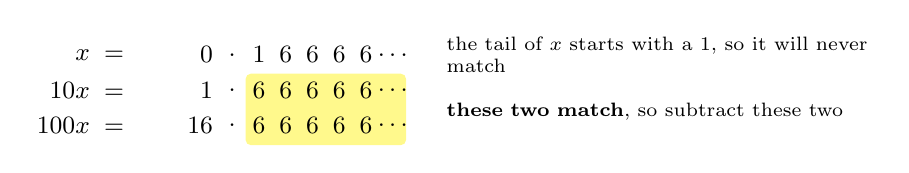
\begin{tikzpicture}[font=\small]
  \fill[yellow!45,rounded corners=2pt] \tailbox{0}{5}{-1.15}{-0.24};
  \drow{0}{$x\;=$}{$0$}{1,6,6,6,6,{$\ldots$}}
  \drow{-0.45}{$10x\;=$}{$1$}{6,6,6,6,6,{$\ldots$}}
  \drow{-0.9}{$100x\;=$}{$16$}{6,6,6,6,6,{$\ldots$}}
  \node[anchor=west,font=\scriptsize,text width=5.4cm] at (2.6,0)
    {the tail of $x$ starts with a $1$, so it will never match};
  \node[anchor=west,font=\scriptsize,text width=5.4cm] at (2.6,-0.72)
    {\textbf{these two match}, so subtract these two};
\end{tikzpicture}
\end{center}

\begin{wex}{turn $0.1\dot{6}$ into a fraction}
\small
\begin{tabular}{@{}ll@{\hspace{1.6em}}l@{}}
\textbf{Step 1 --- introduce $x$} & $x=0.1\dot{6}$, so $x=0.16666\ldots$ &\\[8pt]
\textbf{Step 2 --- shift the place values.} & $10x=1.6666\ldots$
  & shift past the $1$\\[8pt]
 & $100x=16.6666\ldots$ & shift one more place\\[8pt]
\textbf{Step 3 --- subtract.} & $100x-10x=16-1=15$ & so $90x=15$\\[8pt]
\textbf{Step 4 --- solve.} & $x=\dfrac{15}{90}=\dfrac{1}{6}$ &\\
\end{tabular}
\end{wex}

\begin{enumerate}[resume]

\item Fill in the gaps to turn $0.2\dot{7}$ into a fraction.
\begin{itemize}[label={},leftmargin=1.8em,itemsep=12pt,topsep=6pt]
  \item \textbf{Step 1 --- introduce $x$} \hfill $x=0.27777\ldots$
  \item \textbf{Step 2 --- shift the place values.} Shift past the $2$:
        \hfill $10x=\ansline[3cm]$
  \item \hspace*{1.2em}Shift one more place: \hfill $100x=\ansline[3cm]$
  \item \textbf{Step 3 --- subtract.} \hfill $100x-10x=\ansline[3cm]$
  \item \hspace*{1.2em}so \hfill $90x=\ansline[3cm]$
  \item \textbf{Step 4 --- solve.} \hfill $x=\ansline[3cm]$
\end{itemize}

\newpage

\item Turn these into fractions in their simplest form. In (d) the repeating
block is two digits long, so think carefully about which two multiples of $x$
you need.
\begin{multicols}{4}
\begin{enumerate}
  \item $0.4\dot{3}$
  \item $0.58\dot{3}$
  \item $0.08\dot{3}$
  \item $0.1\dot{2}\dot{4}$
\end{enumerate}
\end{multicols}
\vspace{13em}

\item The same four steps work when the number is bigger than $1$. Turn
these into improper fractions in their simplest form.
\begin{multicols}{3}
\begin{enumerate}
  \item $2.\dot{7}$
  \item $1.\dot{4}\dot{5}$
  \item $3.\dot{1}\dot{8}$
\end{enumerate}
\end{multicols}
\vspace{13em}

\item \textbf{Mixed practice.} Decide for yourself what to multiply by each
time. Simplify every answer.
\begin{multicols}{4}
\begin{enumerate}
  \item $0.\dot{8}$
  \item $0.\dot{6}\dot{3}$
  \item $0.2\dot{5}$
  \item $0.\dot{0}2\dot{7}$
  \item $0.7\dot{2}$
  \item $0.\dot{1}\dot{2}$
  \item $0.41\dot{6}$
  \item $0.06\dot{4}$
\end{enumerate}
\end{multicols}
\vspace{13em}

\end{enumerate}

\newpage

\parttitle{5}{Challenges}

\begin{enumerate}[resume]

\item \textbf{The value of $0.\dot{9}$.}
\begin{enumerate}
  \item Use the four steps from Part 2 on $x=0.\dot{9}$. What fraction do
        you get?

        \vspace{12em}
  \item Ella says: ``That has to be wrong. $0.9999\ldots$ is obviously a bit
        less than $1$.'' The number line below marks $0.9$, then $0.99$, then
        $0.999$, and so on. Use it, together with the fact that
        $\frac{1}{3}=0.\dot{3}$, to write a reply to Ella.
\end{enumerate}

\vspace{4pt}
\begin{center}
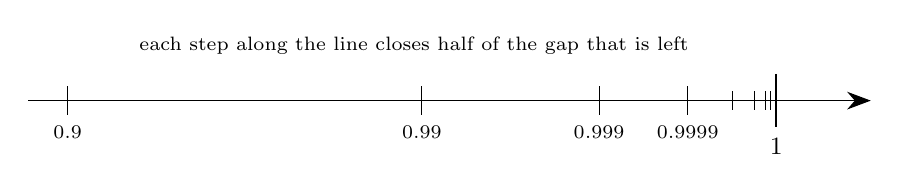
\begin{tikzpicture}[font=\small]
  \node[font=\scriptsize] at (4.4,0.7) {each step along the line closes half of the gap that is left};
  \draw[-{Stealth[length=3mm]}] (-0.5,0) -- (10.2,0);
  \foreach \x/\lab in {0/$0.9$, 4.5/$0.99$, 6.75/$0.999$, 7.875/$0.9999$}{
    \draw (\x,0.18) -- (\x,-0.18);
    \node[below,font=\scriptsize] at (\x,-0.2) {\lab};}
  \foreach \x in {8.44,8.72,8.86,8.93}{\draw (\x,0.12) -- (\x,-0.12);}
  \draw[thick] (9,0.34) -- (9,-0.34);
  \node[below,font=\small] at (9,-0.36) {$1$};
\end{tikzpicture}
\end{center}
\vspace{4pt}

\begin{enumerate}[resume]
  \item What is the largest number that is smaller than $1$? Explain.

        \vspace{14em}
\end{enumerate}

\newpage

\item \textbf{Which fractions recur?} Some fractions give decimals that stop
--- these are called \emph{terminating} decimals --- and some give decimals
that recur forever.
\begin{enumerate}
  \item Complete the table using short division. Circle the terminating ones.

\vspace{3pt}
\begin{center}\small
\begin{tabular}{|c|c|c|c|c|c|}
\hline
\rule{0pt}{2.8em}$\frac{1}{2}=0.5$ & $\frac{1}{3}=$\rule{1.48cm}{0pt} &
$\frac{1}{4}=$\rule{1.48cm}{0pt} & $\frac{1}{5}=$\rule{1.48cm}{0pt} &
$\frac{1}{6}=$\rule{1.48cm}{0pt} & $\frac{1}{7}=$\rule{1.48cm}{0pt}\\
\hline
\rule{0pt}{2.8em}$\frac{1}{8}=$\rule{1.48cm}{0pt} & $\frac{1}{9}=$\rule{1.48cm}{0pt} &
$\frac{1}{10}=$\rule{1.48cm}{0pt} & $\frac{1}{11}=$\rule{1.48cm}{0pt} &
$\frac{1}{12}=$\rule{1.48cm}{0pt} & $\frac{1}{16}=$\rule{1.48cm}{0pt}\\
\hline
\end{tabular}
\end{center}
\vspace{3pt}

  \item Write each terminating denominator as a product of its prime factors.
        What do they all have in common?

        \vspace{9em}
  \item Without dividing, predict whether each of these terminates or recurs,
        and say how you know.
        \[\frac{1}{15}\qquad\frac{1}{40}\qquad\frac{1}{35}\qquad\frac{1}{64}\]

        \vspace{9em}
  \item Why does having only $2$s and $5$s in the denominator make the decimal
        stop? \emph{Hint: what is special about $2\times5$?}

        \vspace{9em}
\end{enumerate}

\newpage

\item \textbf{Sevenths.} One seventh has a repeating block of six digits:
$\dfrac{1}{7}=0.\dot{1}4285\dot{7}$.

\vspace{2pt}
\begin{minipage}[t]{0.58\linewidth}
\begin{enumerate}
  \item Use short division to work out $\frac{2}{7}$, $\frac{3}{7}$,
        $\frac{4}{7}$, $\frac{5}{7}$ and $\frac{6}{7}$ as recurring decimals.

        \vspace{9em}
  \item What do you notice? Use the wheel to describe what happens.

        \vspace{6em}
  \item Use the four steps on $0.\dot{2}8571\dot{4}$ to turn it back into a
        fraction, and check that it agrees with your answer to part (a).

        \vspace{7em}
\end{enumerate}
\end{minipage}\hfill
\begin{minipage}[t]{0.38\linewidth}
\centering
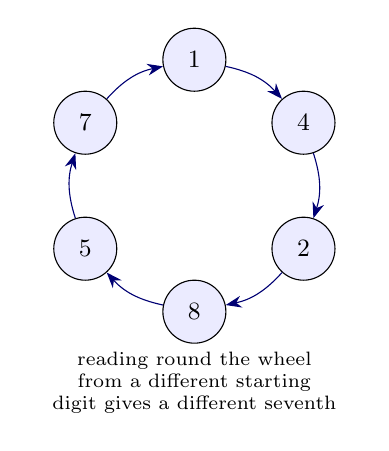
\begin{tikzpicture}[baseline=(current bounding box.north),font=\small]
  \foreach \d [count=\i from 0] in {1,4,2,8,5,7}{
    \node[circle,draw,minimum size=8mm,inner sep=0pt,fill=blue!8]
      (n\i) at ({90-\i*60}:1.6) {\d};}
  \foreach \i/\j in {0/1,1/2,2/3,3/4,4/5,5/0}{
    \draw[-{Stealth[length=2mm]},blue!45!black] (n\i) to[bend left=18] (n\j);}
  \node[font=\scriptsize,text width=4cm,align=center] at (0,-2.5)
    {reading round the wheel from a different starting digit gives a
     different seventh};
\end{tikzpicture}
\end{minipage}

\newpage

\item \textbf{Make your own.}
\begin{enumerate}
  \item Invent a recurring decimal that converts to a fraction with
        denominator $11$. Show that it works.

        \vspace{10em}
  \item Find the recurring decimal that is exactly $\frac{5}{6}$, then use
        the four steps to turn it back into $\frac{5}{6}$.

        \vspace{10em}
  \item Is \emph{every} recurring decimal equal to a fraction? Explain, in
        your own words, why the subtraction always works, whatever recurring
        decimal you start with.

        \vspace{10em}
  \item Ben says: ``$\pi=3.14159\ldots$ goes on forever, so there must be a
        recurring decimal that is exactly equal to $\pi$.'' Use your answer to
        part (c) to explain why Ben is wrong.

        \vspace{10em}
\end{enumerate}

\end{enumerate}

\newpage

\heading{Answers}

{\small
\begin{multicols}{2}
\raggedcolumns
\setlength{\parskip}{4pt}

\textbf{Q1.} (a) $0.55555555$ \quad (b) $0.18181818$ \quad (c) $0.37777777$
\quad (d) $0.20620620$ \quad (e) $0.45151515$ \quad (f) $0.99999999$

\textbf{Q2.} (a) $0.\dot{8}$ \quad (b) $0.\dot{6}\dot{3}$ \quad
(c) $0.2\dot{4}$ \quad (d) $0.\dot{1}5\dot{7}$ \quad (e) $0.91\dot{6}$ \quad
(f) $0.4\dot{0}\dot{5}$

\textbf{Q3.} (a) $0.\dot{4}\dot{5}=0.454545$ and $0.4\dot{5}=0.455555$, so
$0.4\dot{5}$ is bigger --- they agree to two decimal places, but the third
digit is $5$ against $4$. \quad (b) Many answers, for example
$0.\dot{3}\dot{5}=0.353535\ldots$

\textbf{Q4.} $10x=7.7777\ldots$; \; $10x-x=7$; \; $9x=7$; \;
$x=\tfrac{7}{9}$

\textbf{Q5.} $x=0.8888\ldots$; \; $10x=8.8888\ldots$; \;
$10x-x=8$, so $9x=8$; \; $x=\tfrac{8}{9}$

\textbf{Q6.} (a) $\tfrac{2}{9}$ \quad (b) $\tfrac{5}{9}$ \quad
(c) $\tfrac{6}{9}=\tfrac{2}{3}$ \quad (d) $\tfrac{3}{9}=\tfrac{1}{3}$

\textbf{Q7.} The block is $2$ digits long, so multiply by $100$:
$100x=72.727272\ldots$; \; $99x=72$; \; $x=\tfrac{72}{99}=\tfrac{8}{11}$

\textbf{Q8.} (a) $\tfrac{15}{99}=\tfrac{5}{33}$ \quad
(b) $\tfrac{6}{99}=\tfrac{2}{33}$ \quad
(c) $\tfrac{54}{99}=\tfrac{6}{11}$ \quad
(d) $\tfrac{90}{99}=\tfrac{10}{11}$ \quad
(e) $\tfrac{108}{999}=\tfrac{4}{37}$, multiplying by $1000$

\textbf{Q9.} (a) Count the digits in the repeating block. If there are $n$ of
them, multiply by $1$ followed by $n$ zeros, so that the block shifts a whole
number of times and the tails line up again. \quad
(b) Both are right: $\tfrac{12}{99}=\tfrac{4}{33}$. Ben has simplified his,
which is what the question asks for.

\textbf{Q10.} $10x=2.7777\ldots$; \; $100x=27.7777\ldots$; \;
$100x-10x=27-2=25$; \; $90x=25$; \; $x=\tfrac{25}{90}=\tfrac{5}{18}$

\textbf{Q11.} (a) $\tfrac{39}{90}=\tfrac{13}{30}$ \quad
(b) $\tfrac{525}{900}=\tfrac{7}{12}$ \quad
(c) $\tfrac{75}{900}=\tfrac{1}{12}$ \quad
(d) $\tfrac{123}{990}=\tfrac{41}{330}$, using $1000x-10x$

\textbf{Q12.} (a) $\tfrac{25}{9}$ \quad (b) $\tfrac{144}{99}=\tfrac{16}{11}$
\quad (c) $\tfrac{315}{99}=\tfrac{35}{11}$

\textbf{Q13.} (a) $\tfrac{8}{9}$ \quad (b) $\tfrac{63}{99}=\tfrac{7}{11}$
\quad (c) $\tfrac{23}{90}$ \quad (d) $\tfrac{27}{999}=\tfrac{1}{37}$ \quad
(e) $\tfrac{65}{90}=\tfrac{13}{18}$ \quad (f) $\tfrac{12}{99}=\tfrac{4}{33}$
\quad (g) $\tfrac{375}{900}=\tfrac{5}{12}$ \quad
(h) $\tfrac{58}{900}=\tfrac{29}{450}$

\textbf{Q14.} (a) $10x=9.9999\ldots$, so $9x=9$ and $x=\tfrac{9}{9}=1$.
\quad (b) The method is sound, so $0.\dot{9}$ really is $1$. Every step along
the number line closes half of what is left, so the marks get as close to $1$
as you like --- there is no room left between $0.\dot{9}$ and $1$ for them to
be different numbers. Also $\frac{1}{3}=0.\dot{3}$, and multiplying both sides
by $3$ gives $1=0.\dot{9}$. \quad (c) There isn't one. Whatever number you
name below $1$, there is always another number between it and $1$ --- which is
exactly why $0.\dot{9}$ has to \emph{be} $1$ rather than sit just below it.

\textbf{Q15.} (a) $\tfrac{1}{3}=0.\dot{3}$, $\tfrac{1}{4}=0.25$,
$\tfrac{1}{5}=0.2$, $\tfrac{1}{6}=0.1\dot{6}$,
$\tfrac{1}{7}=0.\dot{1}4285\dot{7}$, $\tfrac{1}{8}=0.125$,
$\tfrac{1}{9}=0.\dot{1}$, $\tfrac{1}{10}=0.1$,
$\tfrac{1}{11}=0.\dot{0}\dot{9}$, $\tfrac{1}{12}=0.08\dot{3}$,
$\tfrac{1}{16}=0.0625$. The terminating ones are
$\tfrac{1}{2},\tfrac{1}{4},\tfrac{1}{5},\tfrac{1}{8},\tfrac{1}{10},
\tfrac{1}{16}$. \quad
(b) $2$, $2^2$, $5$, $2^3$, $2\times5$, $2^4$ --- every one is built out of
$2$s and $5$s only. \quad
(c) $\tfrac{1}{15}$ recurs, since $15=3\times5$ and the $3$ is not allowed;
$\tfrac{1}{40}$ terminates, since $40=2^3\times5$; $\tfrac{1}{35}$ recurs,
since $35=5\times7$; $\tfrac{1}{64}$ terminates, since $64=2^6$. \quad
(d) A terminating decimal is just a fraction over $10$, $100$, $1000$,
\ldots, and $10=2\times5$. So a fraction can be rewritten over a power of ten
exactly when its denominator is built from $2$s and $5$s; any other prime
factor can never be cancelled away.

\textbf{Q16.} (a) $\tfrac{2}{7}=0.\dot{2}8571\dot{4}$,
$\tfrac{3}{7}=0.\dot{4}2857\dot{1}$, $\tfrac{4}{7}=0.\dot{5}7142\dot{8}$,
$\tfrac{5}{7}=0.\dot{7}1428\dot{5}$, $\tfrac{6}{7}=0.\dot{8}5714\dot{2}$.
\quad (b) They all use the same six digits in the same cyclic order,
$1\to4\to2\to8\to5\to7\to1$; each seventh simply starts at a different place
on the wheel. \quad (c) The block is $6$ digits long, so multiply by
$1\,000\,000$: this gives $999\,999x=285\,714$, so
$x=\tfrac{285714}{999999}=\tfrac{2}{7}$, dividing top and bottom by
$142\,857$.

\textbf{Q17.} (a) Many answers. For example $0.\dot{2}\dot{7}$ gives
$99x=27$, so $x=\tfrac{27}{99}=\tfrac{3}{11}$; any two-digit block that is a
multiple of $9$ but not of $11$ will do. \quad
(b) $\tfrac{5}{6}=0.8\dot{3}$, and checking: $100x-10x=83-8=75$, so $90x=75$
and $x=\tfrac{75}{90}=\tfrac{5}{6}$. \quad
(c) Yes. Whatever the decimal, shifting it by the length of the repeating
block always produces a second number with an identical tail, so the
subtraction always leaves a whole number. That gives an equation of the form
(whole number)$\,\times x=$ (whole number), and dividing gives a fraction.
\quad (d) $\pi$ is not a fraction, and part (c) shows that every recurring
decimal is one. So no recurring decimal can equal $\pi$: its digits go on
forever without ever settling into a repeating block.

\end{multicols}
}

\end{document}
